\documentclass[12pt]{article}
\usepackage{amsmath}
\usepackage{amssymb}
\usepackage[letterpaper,margin=0.85in,centering]{geometry}
\usepackage{fancyhdr}
\usepackage{enumerate}
\usepackage{lastpage}
\usepackage{multicol}
\usepackage{graphicx}

\reversemarginpar

\pagestyle{fancy}
\cfoot{}
\lhead{Math 1410}\chead{Worksheet \# 2}\rhead{September 21/22, 2016}
%\rfoot{Total: 10 points}
%\chead{{\bf Name:}}
\newcommand{\points}[1]{\marginpar{\hspace{24pt}[#1]}}
\newcommand{\skipline}{\vspace{12pt}}
%\renewcommand{\headrulewidth}{0in}
\headheight 30pt

\newcommand{\di}{\displaystyle}
\newcommand{\abs}[1]{\lvert #1\rvert}
\newcommand{\len}[1]{\lVert #1\rVert}
\renewcommand{\i}{\mathbf{i}}
\renewcommand{\j}{\mathbf{j}}
\renewcommand{\k}{\mathbf{k}}
\newcommand{\R}{\mathbb{R}}
\newcommand{\aaa}{\mathbf{a}}
\newcommand{\bbb}{\mathbf{b}}
\newcommand{\ccc}{\mathbf{c}}
\newcommand{\dotp}{\boldsymbol{\cdot}}
\newcommand{\bbm}{\begin{bmatrix}}
\newcommand{\ebm}{\end{bmatrix}}                   
                  
\begin{document}
{\bf \large Name:} \hspace{2.5in} {\bf Tutorial day and time:}

\bigskip

{\bf Number of the {\em completed} problem you want feedback on:}

\bigskip

%\author{Instructor: Sean Fitzpatrick}
\thispagestyle{fancy}
%\noindent{{\bf Name and student number:}}

 \begin{enumerate}
 \item Calculate the four 4th roots of the complex number $z=-2\sqrt{3}+2i$.

\vspace{2.75in}


 \item  Let $P=(1,0,-2)$, $Q=(-3,2,4)$, and $R=(0,5,-1)$ be points in $\R^3$.
\begin{enumerate}
 \item Calculate the vectors $\vec{u}=\overrightarrow{PQ}$, $\vec{v}=\overrightarrow{QR}$, and $\vec{w}=\overrightarrow{PR}$.

\vspace{1.75in}

 \item Check that $\vec{u}+\vec{v} = \vec{w}$.

\vspace{0.75in}

 \item Explain, with a diagram, why your result in part (b) makes sense. (You do not have to accurately plot the points $P,Q,R$.)


\end{enumerate}
\newpage

\item Let $\vec{a} = \langle 2,-4,3\rangle$, $\vec{b} = \langle -5, 2, 7\rangle$, and $\vec{c} = \langle 1,0,-3\rangle$. Calculate the following:
\begin{enumerate}
 \item $4\vec{a}-3\vec{b}$

\vspace{2.5cm}

 \item $\len{3\vec{c}}$

\vspace{2.5cm}

 \item $3\len{\vec{c}}$

\vspace{2.5cm}

 \item $\vec{a}\dotp (2\vec{b}-\vec{c})$

\vspace{3cm}

 \item $2(\vec{a}\dotp \vec{b}) - \vec{a}\dotp\vec{c}$
\end{enumerate}

\vspace{3cm}

\item Referring to the diagram below, argue that the indicated distance $d$ is given by $d = \dfrac{\vec{a}\dotp\vec{b}}{\len{\vec{a}}}$.
\begin{flushleft}
 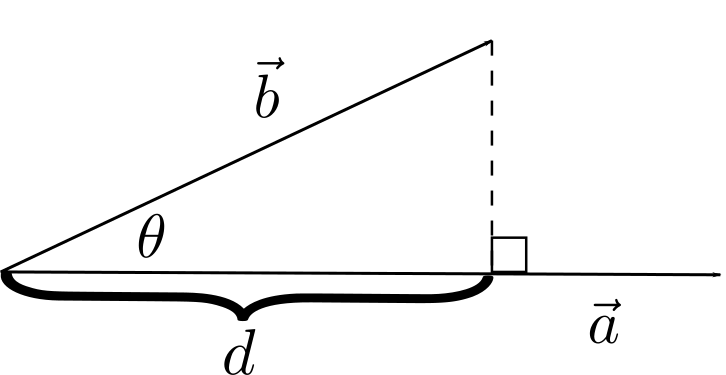
\includegraphics[width=2in]{WS2_proj}
\end{flushleft}




 \end{enumerate}\end{document}